\documentclass[a4paper,twoside]{article}
\usepackage{amssymb}
\usepackage{amsthm}
\usepackage{amsmath}
\usepackage{mathtools}
\usepackage{enumerate}
\usepackage{hyperref}
\usepackage{tabstackengine}
\usepackage{indentfirst}
\usepackage{verbatim}
\usepackage{makeidx}
\usepackage{graphicx}
\usepackage{enumerate}
\usepackage{color}
\usepackage{colonequals}
\usepackage{listings}
\usepackage{mathrsfs}
\usepackage[top=1.1in,right=1.1in,left=1.1in,bottom=1.1in]{geometry}
\usepackage[numbers]{natbib}
\usepackage{fancyhdr}
\usepackage{pdfpages}
\usepackage{mwe} 
\usepackage{wrapfig}
\usepackage{listings}
\usepackage{xcolor}

\definecolor{codegreen}{rgb}{0,0.6,0}
\definecolor{codegray}{rgb}{0.5,0.5,0.5}
\definecolor{codepurple}{rgb}{0.58,0,0.82}
\definecolor{backcolour}{rgb}{0.95,0.95,0.92}

\raggedbottom
\lstdefinestyle{mystyle}{
    backgroundcolor=\color{backcolour},   
    commentstyle=\color{codegreen},
    keywordstyle=\color{magenta},
    numberstyle=\tiny\color{codegray},
    stringstyle=\color{codepurple},
    basicstyle=\ttfamily\footnotesize,
    breakatwhitespace=false,
    breaklines=true,                 
    captionpos=b,                    
    keepspaces=true,                 
    numbers=left,                    
    numbersep=5pt,                  
    showspaces=false,                
    showstringspaces=false,
    showtabs=false,                  
    tabsize=2
}

\lstset{style=mystyle}

\hypersetup{
    colorlinks=true,
    linkcolor=blue,
    filecolor=magenta,
    urlcolor=cyan,
    pdftitle={Sharelatex Example},
    % bookmarks=true,
    pdfpagemode=FullScreen,
}
\DeclareMathOperator{\spn}{span}
\renewcommand{\vec}[1]{\mathbf{#1}}
\pagestyle{fancy}
\fancyhead{}
\fancyhead{\lhead{\small{\nouppercase{\textsc{\leftmark}}}}}
\makeindex
\setlength{\parskip}{0.1cm}
\newtheorem{theorem}{Theorem}[section]
\newtheorem{lemma}[theorem]{Lemma}
\newtheorem{proposition}[theorem]{Proposition}
\newtheorem{corollary}[theorem]{Corollary}
\newtheorem{example}[theorem]{Example}
\newtheorem{definition}[theorem]{Definition}
\newtheorem{algorithm}[theorem]{Algorithm}
\newtheorem{remark}[theorem]{Remark}
\newtheorem{conjecture}[theorem]{Conjecture}
\numberwithin{equation}{section}
\newcommand\myeq{\mathrel{\overset{\makebox[0pt]{\mbox{\normalfont\footnotesize\sffamily by (\ref{min_evalue}) }}}{=}}} \newcommand\mygeq{\mathrel{\overset{\makebox[0pt]{\mbox{\normalfont\footnotesize\sffamily by (\ref{min_evalue}) }}}{\geq}}}


%\usepackage{xcolor}

%\pagecolor[rgb]{0,0,0} %black

%\color[rgb]{0.7,0.7,0.7} %grey



 \providecommand{\given}{}
\newcommand{\setseparator}{% used only in \Set
	\mathrel{}
	\mathclose{}
	\delimsize|
	\mathopen{}
	\mathrel{}
}
\DeclarePairedDelimiterX{\Set}[1]{\lbrace}{\rbrace}{%
	\renewcommand{\given}{\setseparator}%
	#1%
}

\newcommand{\longsetdescription}[2][.55\displaywidth]{\parbox{#1}{#2}}

\hyphenpenalty=10000



\begin{document}
%\includepdf[pages=-,pagecommand={},width=\textwidth]{declaration.pdf}



\title{MIT 6.004 Computational Structures} \author{} \date{\today} \maketitle \thispagestyle{empty}

% %TC:ignore
% \begin{abstract}
% \end{abstract}
%TC:endignore


\pagenumbering{roman}
\setcounter{page}{1}

\tableofcontents
\newpage
\setcounter{section}{0}
\pagenumbering{arabic}
\setcounter{page}{1}
\section{Introduction}
\label{Introduction}
This course offers an introduction to the engineering of digital systems. Starting with MOS transistors,
the course develops a series of building blocks - logic gates, combinational and sequential circuits, finite-state machines, computers and finally complete systems. Both hardware and software mechanisms are explored through a series of design examples. This document contains my lecture notes for \href{https://ocw.mit.edu/courses/6-004-computation-structures-spring-2017/pages/syllabus/} Computational Structures. Youtube video lectures are uploaded \href{https://www.youtube.com/watch?v=R0tFDXBZvKI&list=PLUl4u3cNGP62WVs95MNq3dQBqY2vGOtQ2&ab_channel=MITOpenCourseWare}{here}.

\section{Lectures}
\subsection{Lecture 1: Basics of information}
\label{Lecture 1}
\subsubsection{What is information?}
\label{What is information?}
\begin{definition}
    Define information as data communicated or received that resolves uncertainty about a particular
     fact or circumstance
\end{definition}
In other words, after receiving the data we'll know more about that particular fact or circumstance.
 The greater the uncertainty resolved by the data, the more information the data has conveyed. More formally:
\begin{definition}
    Assume our application deals with circumstances where there are a finite number N of distinct
    choices modelled by a random variable $X$ with possible outcomes $x_1, x_2 ... x_N$.
    Then the information we receive when we learn $X$ has taken value $x_i$ is:
    \begin{equation}
        I(x_i) = log_2(\dfrac{1}{p_i}) bits
    \end{equation}
\end{definition}
The information is proportional with the reversed probability, i.e The less likely event occur the
 more info we get.
\begin{center}
    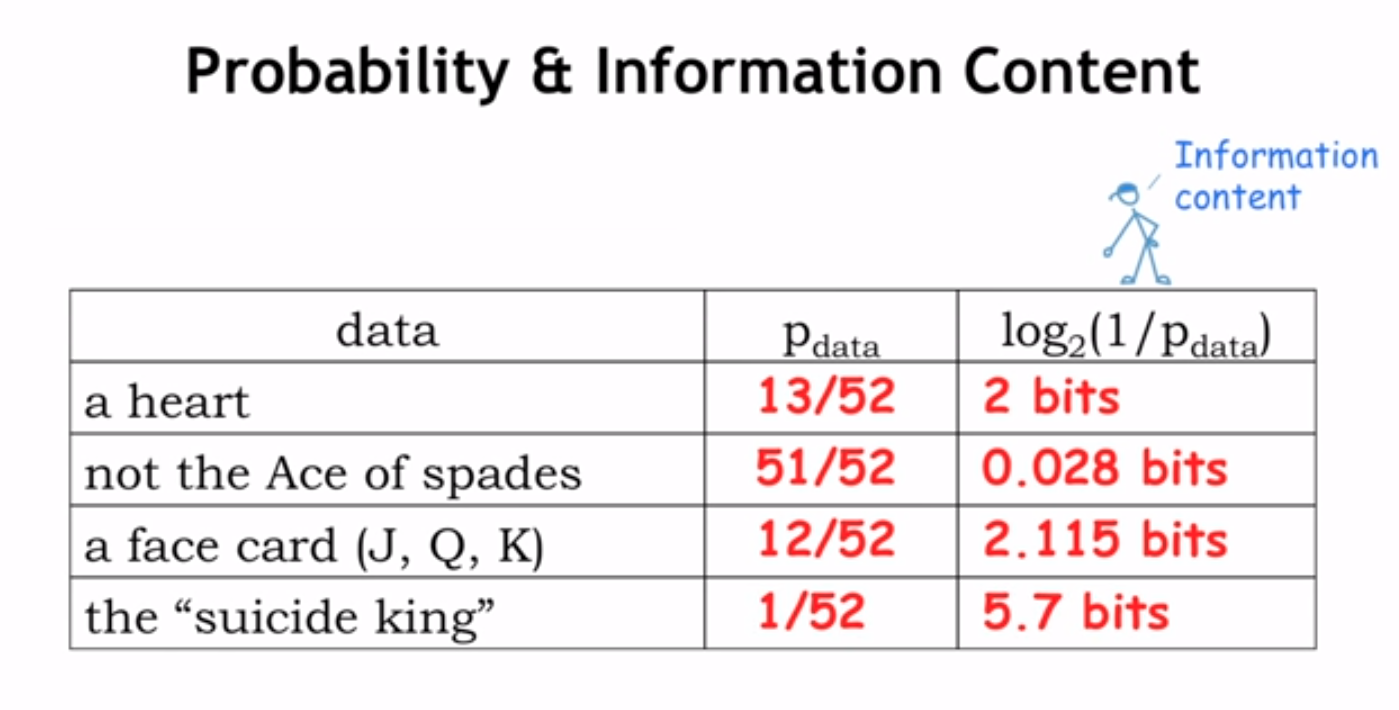
\includegraphics[scale=0.2]{assets/prob_information.png}
\end{center}
In the above example it makes sense that revealing a heart is 2 bits as in total we have 4 colors and
we need 2 bits to be able to capture/encode all colors. Another example is flipping a coin where the
 result of of throw (e.g. heads) would give us $log_2(2) = 1$ bit of information. Indeed with 1 bit
 we can encode binary outcome like head/tail. In practice the above table should round up the bits
  to the nearest integer.

\begin{definition}
    In information theory, the \textbf{entropy} $H(X)$ is the average amount of information contained
    in each piece of data received about the value of X (expected number of bits):
    \begin{equation}
        H(X) = \mathbf{E}(I(X)) = \sum p_i log_2(\dfrac{1}{p_i})
    \end{equation}
\end{definition}

\begin{center}
    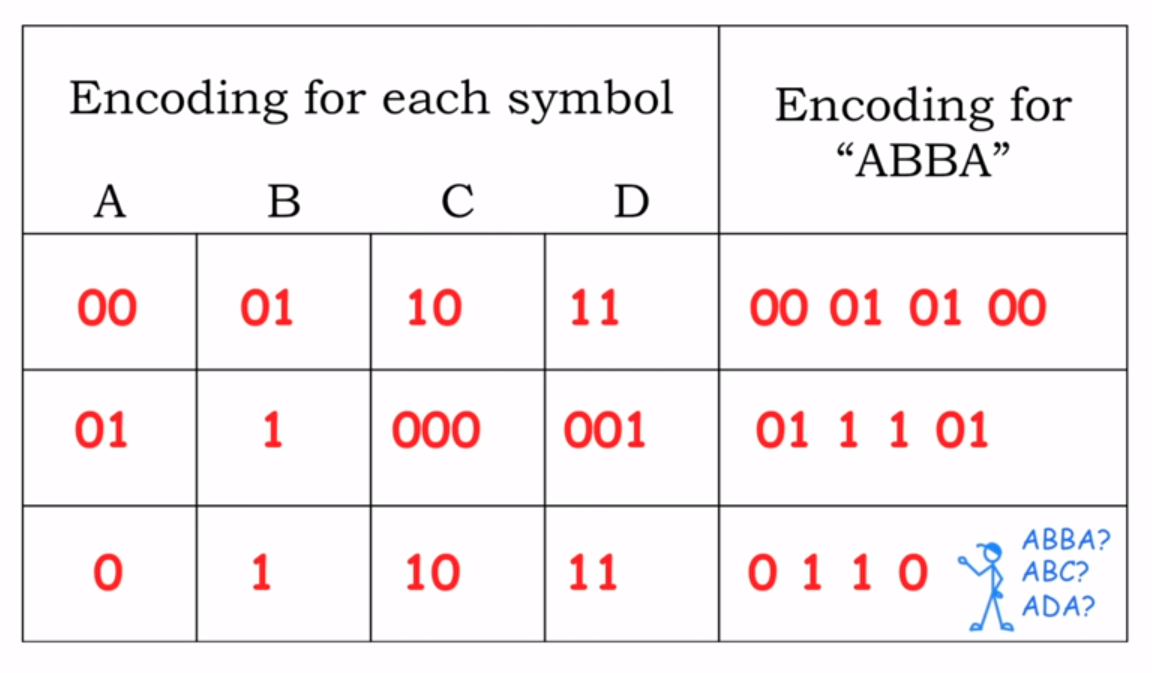
\includegraphics[scale=0.2]{assets/encodings.png}
\end{center}

\subsubsection{Encodings}

\begin{definition}
    An \textbf{encoding} is an unambiguous mapping between bit strings and the set of possible data.
     I.e. should encode each possible symbol differently (A = 00, B = 01, C = 10, D = 11) ->
     ABBA = 00 01 01 00.
\end{definition}

his is called a fixed-length encoding since the bit strings used to represent the symbols all have the
same length. The encoding for the message “ABBA” would be “00 01 01 00”. And we can run the process
 backwards: given a bit string and the encoding key, we can look up the next bits in the bit string,
 using the key to determine the symbol they represent. “00” would be decoded as “A,” “01” as B and so on.

As shown in the second encoding in the table, we can use a variable-length encoding, where the symbols
are encoded using bit strings of different lengths. here “A” is encoded as “01,” “B” as “1”, “C” as “000”
and “D” = “001.”. “ABBA” would be encoded as “01 1 1 01.” We'll see that carefully constructed variable-length
 encodings are useful for the efficient encoding of messages where the symbols occur with different
 probabilities.

\begin{center}
    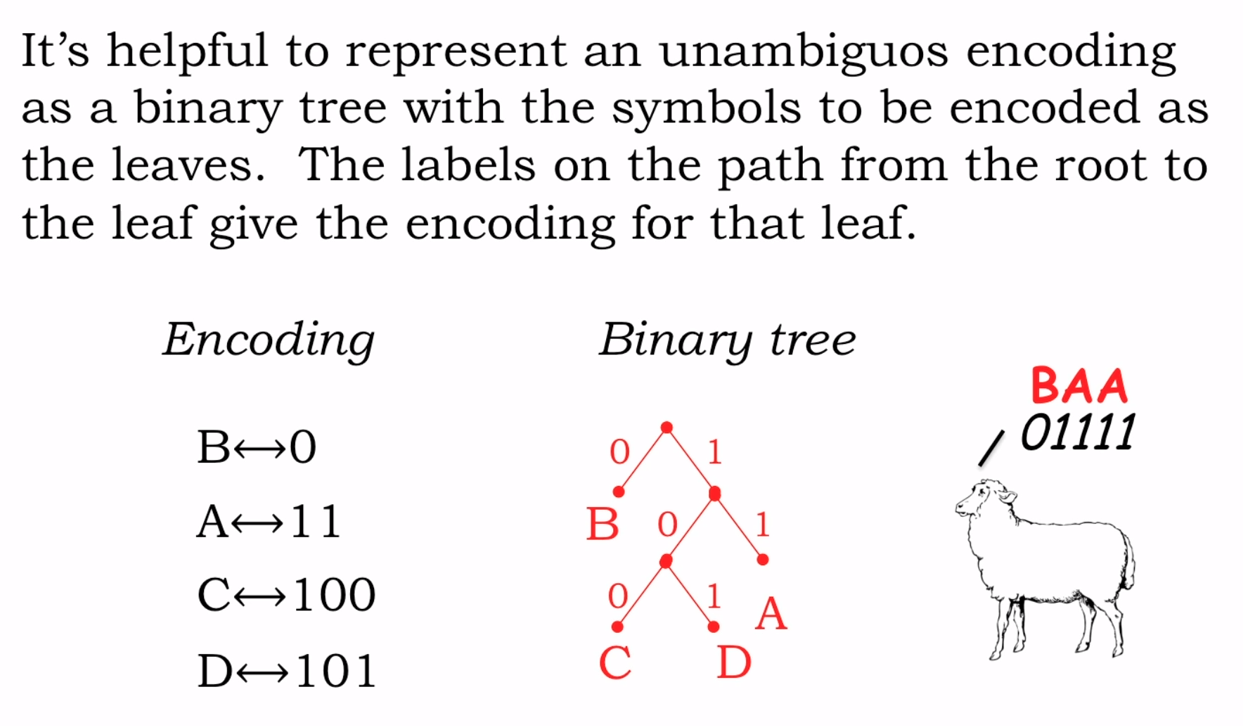
\includegraphics[scale=0.3]{assets/encodings_tree.png}
\end{center}
Graphically we can represent an unambiguous encoding as a binary tree, labeling the branches from each
tree node with “0” and “1,” placing the symbols to be encoded as the leaves of the tree. If you build a
binary tree for a proposed encoding and find that there are no symbols labeling interior nodes and exactly
one symbol at each leaf, then your encoding is good to go!\newline
If the symbols we are trying to encode occur with equal probability (or if we have no a priori reason
to believe otherwise), then we'll use a fixed-length encoding, where all leaves in the encoding's binary
 tree are the same distance from the root. Fixed-length encodings have the advantage of supporting random
 access, where we can figure out the Nth symbol of the message by simply skipping over the required number
 of bits. For example, in a message encoded using the fixed-length code shown here, if we wanted to determine
 the third symbol in the encoded message, we would skip the 4 bits used to encode the first two symbols and
 start decoding with the 5th bit of message. Note entropy here is:
\begin{equation}
    \sum \dfrac{1}{n} log_2(\dfrac{1}{1/n}) = log_2(N)
\end{equation}
\begin{example}
    In binary-coded decimal, each digit of a decimal number is encoded separately. Since there are 10
    different decimal digits, we'll need to use a 4-bit code to represent the 10 possible choices.
     The associated entropy is $log_2(10)$, which is 3.322 bits. We can see that our chosen encoding
     is inefficient in the sense that we'd use more than the minimum number of bits necessary to encode,
     say, a number with 1000 decimal digits: our encoding would use 4000 bits, although the entropy
     suggests we *might* be able to find a shorter encoding, say, 3400 bits, for messages of length 1000.
\end{example}

\begin{example}
    Integer numbers will use a base 2 representation using the two binary digits. I.e. 5  has binary
    encoding 1001.
\end{example}
With this N-bit representation, the smallest number that can be represented is 0
(when all the binary digits are 0) and the largest number is $2**N -1$ (when all the binary digits are 1).
 Many digital systems are designed to support operations on binary-encoded numbers of some fixed size, e.g.,
  choosing a 32-bit or a 64-bit representation, which means that they would need multiple operations when
   dealing with numbers too large to be represented as a single 32-bit or 64-bit binary string. \newline
Long strings of binary digits are tedious and error-prone to transcribe, so let's find a more
convenient notation, ideally one where it will be easy to recover the original bit string without
 too many calculations. A good choice is to use a representation based on a radix that's some higher power
  of 2, so each digit in our representation corresponds to some short contiguous string of binary bits.
  A popular choice these days is a radix-16 representation, called hexadecimal or “hex” for short, where
  each group of 4 binary digits is represented using a single hex digit.

\begin{center}
    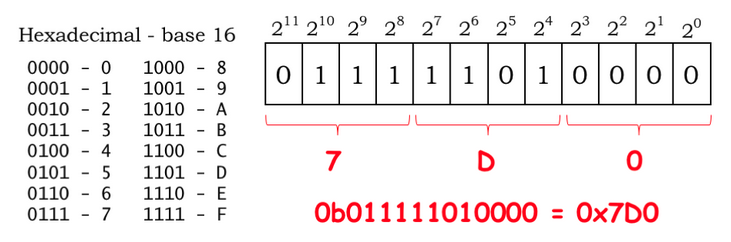
\includegraphics[scale=0.4]{assets/hexadecimal_notation.png}
\end{center}
To convert a binary number to hex, group the binary digits into sets of 4, starting with the
least-significant bit (that's the bit with weight ). Then use the table to convert each 4-bit
 pattern into the corresponding hex digit: “0000” is the hex digit “0”, “1101” is the hex digit “D,”
  and “0111” is the hex digit “7”. The resulting hex representation is “7D0.” To prevent any confusion,
  we'll use a special prefix “0x” to indicate when a number is being shown in hex, so we'd write “0x7D0”
   as the hex representation for the binary number “0111 1101 0000.” This notation convention is used
   by many programming languages for entering binary bit strings. \newline
Finally we encode signed integers.
\begin{proposition}
    In decimal notation, the convention is to precede the number with a “+” or “-” to indicate whether
    it's positive or negative, usually omitting the “+” to simplify the notation for positive numbers.
\end{proposition}
We use similar strategy when presenting numbers in binary notation where we put a 1 in front for
negative and 0 for positive:
\begin{center}
    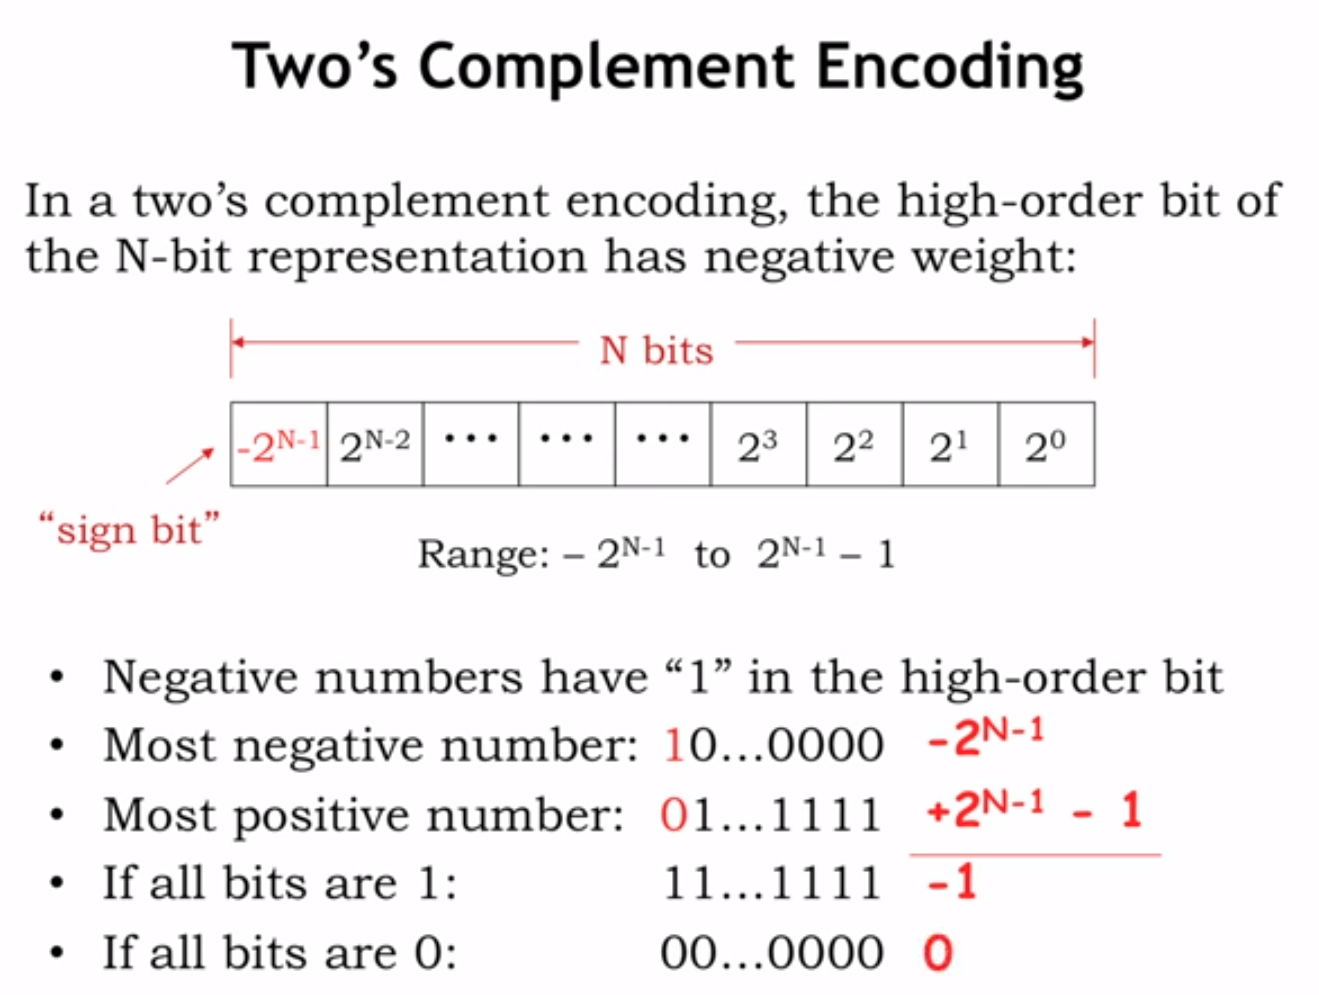
\includegraphics[scale=0.2]{assets/twos_complement.png}
\end{center}

\begin{center}
    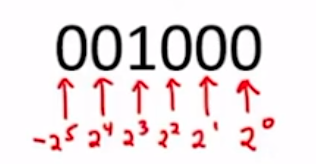
\includegraphics[scale=0.2]{assets/twos.png}
\end{center}
Let's see what happens when we add the N-bit values for -1 and 1, keeping an N-bit answer. In the
rightmost column, 1 plus 1 is 0, carry the 1. In the second column, the carry of 1 plus 1 plus 0 is 0,
carry the 1. And so on — the result is all zero's, the representation for 0… perfect! Notice that we
 just used ordinary binary addition, even when one or both of the operands are negative.
 Two's complement is perfect for N-bit arithmetic!

\begin{center}
    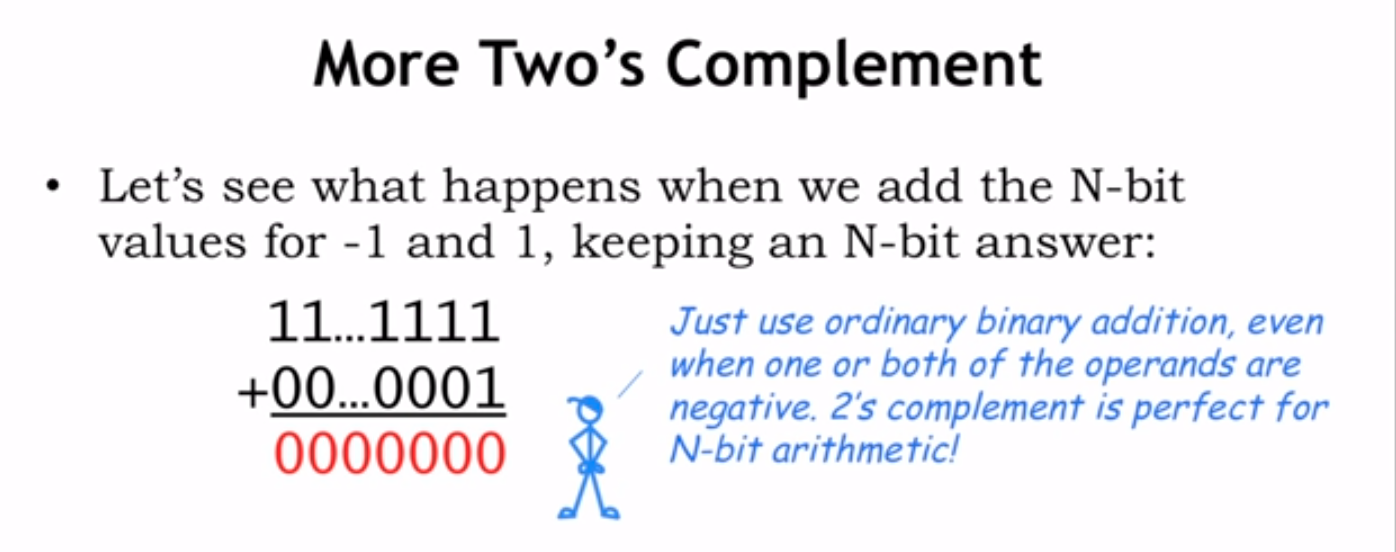
\includegraphics[scale=0.2]{assets/oneplusone.png}
\end{center}

\begin{definition}
    A number $x$ and its two's complement sum to $2^N$.
\end{definition}
Fixed-length encodings work well when all the possible choices have the same information content,
 i.e., all the choices have an equal probability of occurring. If those choices don't have the
 same information content, we can do better.

\begin{center}
    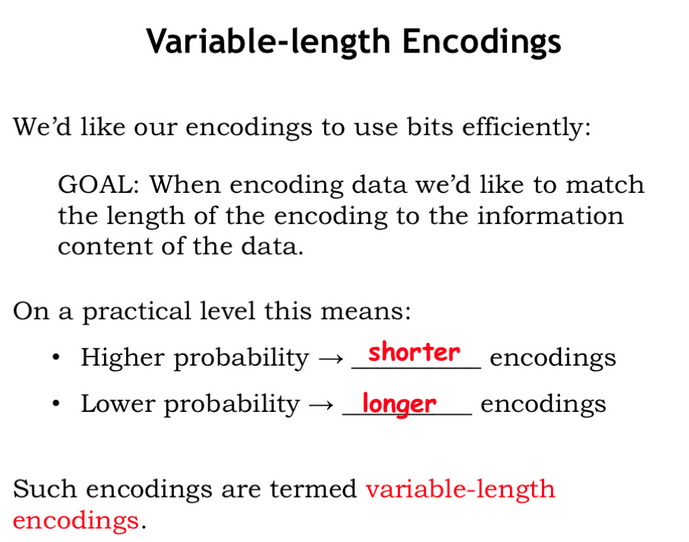
\includegraphics[scale=0.3]{assets/variable_length_encoding.png}
\end{center}
Consider the expected length of an encoding, computed by considering each event $x_i$  to be encoded,
 and weighting the length of its encoding by $p_i$, the probability of its occurrence. By “doing better”
  we mean that we can find encodings that have a shorter expected length than a fixed-length encoding.
  Ideally we'd like the expected length of the encoding for the $x_i$ to match the entropy H(X), which
  is the expected information content. Next we consider an example encoding.
\begin{center}
    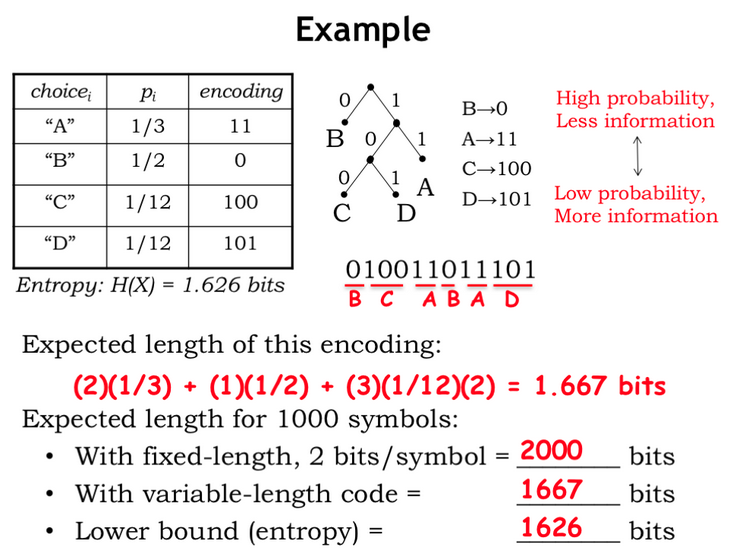
\includegraphics[scale=0.3]{assets/example_encoding.png}
\end{center}
Could another variable-length encoding have done better? In general, it would be nice to have a
 systematic way to generate the best-possible variable-length code

\subsubsection{Huffman's encoding}
\begin{center}
    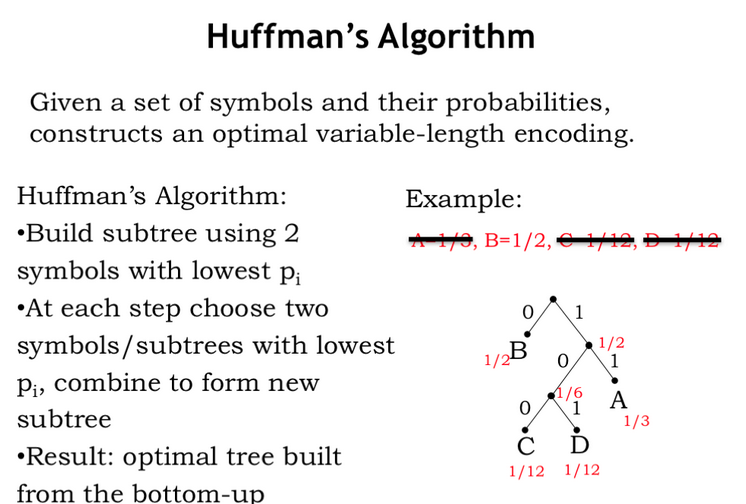
\includegraphics[scale=0.3]{assets/huffman.png}
\end{center}
Given a set of symbols and their probabilities, Huffman's Algorithm tells us how to construct an
optimal variable-length encoding. By “optimal” we mean that, assuming we're encoding each symbol
 one-at-a-time, no other variable-length code will have a shorter expected length.

The algorithm builds the binary tree for the encoding from the bottom up. Start by choosing the two
symbols with the smallest probability (which means they have highest information content and should
have the longest encoding). If anywhere along the way, two symbols have the same probability, simply
choose one arbitrarily. In our running example, the two symbols with the lowest probability are C and D.
\newline
Combine the symbols as a binary subtree, with one branch labeled “0” and the other “1.” It doesn't
matter which labels go with which branch. Remove C and D from our list of symbols, and replace
them with the newly constructed subtree, whose root has the associated probability of 1/6, the sum of
 the probabilities of its two branches.
\newline
Now continue, at each step choosing the two symbols and/or subtrees with the lowest probabilities,
combining the choices into a new subtree. At this point in our example, the symbol A has the probability
1/3, the symbol B the probability 1/2 and the C/D subtree probability 1/6. So we'll combine A with the
C/D subtree.
\newline
On the final step we only have two choices left: B and the A/C/D subtree, which we combine in a new
subtree, whose root then becomes the root of the tree representing the optimal variable-length code.
Happily, this is the code we've been using all along! \newline
“Optimal” sounds pretty good! Does that mean we can't do any better? Well, not by encoding symbols
one-at-a-time. But if we want to encode long sequences of symbols, we can reduce the expected length
of the encoding by working with, say, pairs of symbols instead of only single symbols.
The table below shows the probability of pairs of symbols from our example. If we use Huffman's A
lgorithm to build the optimal variable-length code using these probabilities, it turns out the expected
length when encoding pairs is 1.646 bits/symbol. This is a small improvement on the 1.667 bits/symbols
when encoding each symbol individually. And we'd do even better if we encoded sequences of length 3,
and so on.\newline
Modern file compression algorithms use an adaptive algorithm to determine on-the-fly which sequences
occur frequently and hence should have short encodings. They work quite well when the data has many
repeating sequences, e.g., natural language data where some letter combinations or even whole words
occur again and again. Compression can achieve dramatic reductions from the original file size.
If you'd like to learn more, look up “LZW” on Wikipedia to read the Lempel-Ziv-Welch data compression
algorithm. \newline
\subsubsection{Error Detection and Correction}
What is Error?/newline
Error is a condition when the output information does not match with the input information.
During transmission, digital signals suffer from noise that can introduce errors in the binary bits
travelling from one system to other. That means a 0 bit may change to 1 or a 1 bit may change to 0.
Whenever a message is transmitted, it may get scrambled by noise or data may get corrupted. To avoid
this, we use error-detecting codes which are additional data added to a given digital message to
help us detect if an error occurred during transmission of the message. A simple example of
error-detecting code is parity check. To detect and correct the errors, additional bits are added
to the data bits at the time of transmission.
\begin{itemize}
    \item The additional bits are called parity bits. They allow detection or correction of the errors.
    \item The data bits along with the parity bits form a code word.
\end{itemize}
\begin{proposition}
    The simplest error checking is \textbf{parity check}. It is the simplest technique for detecting
     and correcting errors.
    The MSB of an 8-bits word is used as the parity bit and the remaining 7 bits are used as data or
    message bits. The parity of 8-bits transmitted word can be either even parity or odd parity.
    The parity bit is set by the user and then we transmit the data. If the receiver gets data with
    1 single bit error we would catch it from the parity bit (which remains unchanged - it is not send
    the user knows it in his head).
\end{proposition}
\begin{definition}
    The Hamming distance between two number is the number of bits they differ (i.e. XOR).
\end{definition}
\begin{definition}
    To detect and correct the errors, additional bits are added to the data bits at the time of transmission.
    \begin{itemize}
        \item  The additional bits are called parity bits. They allow detection or correction of
              the errors.
        \item  The data bits along with the parity bits form a code word.
    \end{itemize}
\end{definition}
In order to capture 1 bit error we needed the input and output to have at least 2 Hammer distance.
In general, to detect some number of $E$ errors, we need a minimum Hamming distance of $E+1$ between
 code words. To correct $E$ errors, we need a minimum Hamming distance of $2E+1$, see more
 \href{https://www.youtube.com/watch?v=2IQxigpPMns&list=PLUl4u3cNGP62WVs95MNq3dQBqY2vGOtQ2&index=16&ab_channel=MITOpenCourseWare}{here}.

\subsection{Lecture 2 The Digital Abstraction}
In the previous lecture, we discussed how to encode information as sequences of bits. In this lecture,
we turn our attention to finding a useful physical representation for bits, our first step in building
devices that can process information. \newline
What makes a good bit, i.e., what properties do we want our physical representation of bits to have?
\begin{itemize}
    \item We want bits to be small and inexpensive as we will be carrying lots of them.
    \item We'd like our representation of bits to make it easy to quickly access, transform, combine,
          transmit and store the information they encode.
\end{itemize}
We'd certainly like our bits to be stable over long periods of time — once a 0, always a 0!
The Rosetta Stone, a decree from the Egyptian King Ptolemy V, was created in 196 BC and encoded the
information needed for archeologists to start reliably deciphering Egyptian hieroglyphics almost 2000
years later. This is one way to have a physical representaion of data. But, the very property that
makes stone engravings a stable representation of information makes it difficult to manipulate the
information (that's why we have the second item in the list above). So instead of representing
information on heavy stones, we'd  represent bits using the electrical phenomenon associated
with charged particles.  The presence of charged particles creates differences in electrical
potential energy we can measure as voltages, and the flow of charged particles can be measured
as currents. We can also encode information using the phase and frequency of electromagnetic
fields associated with charged particles — these latter two choices form the basis for wireless
communication
\subsubsection{Using voltages to represent the information}
\begin{definition}
    Voltage is the pressure from an electrical circuit's power source that pushes charged electrons
    (current) through a conducting loop. In brief, voltage = pressure, and it is measured in volts (V).
    In electricity's early days, voltage was known as electromotive force (emf).
\end{definition}

\begin{remark}
    Some translations of terms: circuit = shema, current = tok, voltage = voltaj.
\end{remark}
\begin{center}
    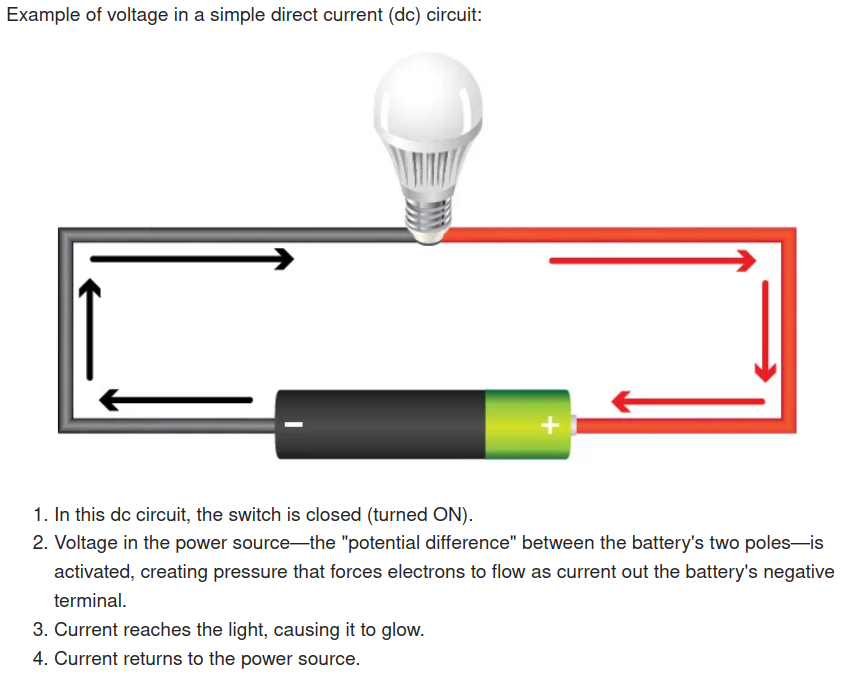
\includegraphics[scale=0.4]{assets/example_voltage.png}
\end{center}
Voltage and the term "potential difference" are often used interchangeably. Potential difference might
be better defined as the potential energy difference between two points in a circuit. The amount of
difference (expressed in volts) determines how much potential energy exists to move electrons from one
specific point to another. The quantity identifies how much work, potentially, can be done through the
circuit. \newline

In this course, we'll use voltages to represent bits. For example, we might choose 0 V to represent
a 0-bit and 1 V to represent a 1-bit. To represent sequences of bits we can use multiple voltage
measurements, either from many different wires, or as a sequence of voltages over time on a single wire.

A representation using voltages has many advantages: electrical outlets provide an inexpensive and
mostly reliable source of electricity and, for mobile applications, we can use batteries to supply
what we need. For more than a century, we've been accumulating considerable engineering knowledge
about voltages and currents. We now know how to build very small circuits to store, detect and manipulate
 voltages. And we can make those circuits run on a very small amount of electrical power. In fact, we can design circuits that require close to zero power dissipation in a steady state if none of the encoded information is changing.
\begin{remark}
    Basically, the motherboard (circuit) where all the work is done by the computer uses physics and
    electrical engineering knowledge to store, transform, maintain, manipulate information which we
    call bits but is physically voltages.
\end{remark}
\begin{example}
    Consider the problem of using voltages to represent the information in a black-and-white image.
    Each (x,y) point in the image has an associated intensity: black is the weakest intensity, white
     the strongest. An obvious voltage-based representation would be to encode the intensity as a voltage,
      say 0V for black, 1V for white, and some intermediate voltage for intensities in-between.
\end{example}
With $N$ bits, we need to be able to distinguish a total $2^N$ voltages in the range of 0V to 1V.
For example, for $N = 2$, we'd need to be able to distinguish between four possible voltages. That
 doesn't seem too hard — an inexpensive volt-meter would let us easily distinguish between 0V, 1/3V,
  2/3V and 1V.
\begin{center}
    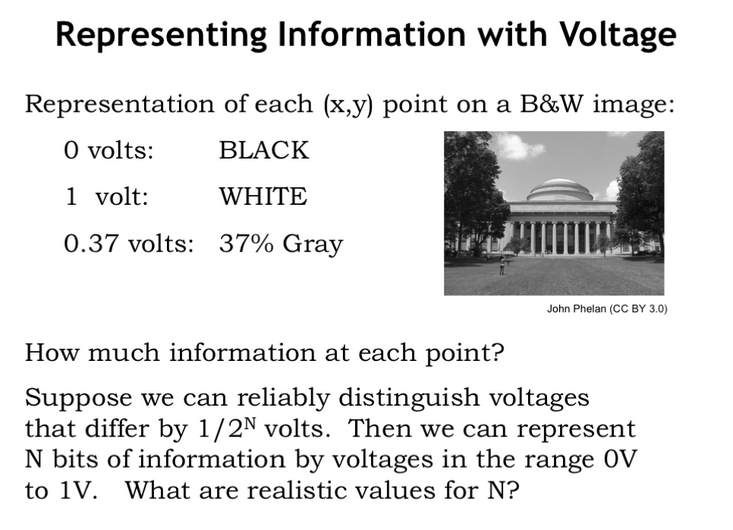
\includegraphics[scale=0.4]{assets/info_voltage.png}
\end{center}
In theory, N can be arbitrarily large. In practice, we know it would be quite challenging to make
measurements with, say, a precision of 1-millionth of a volt and probably next to impossible if we
wanted a precision of 1-billionth of a volt.
\begin{center}
    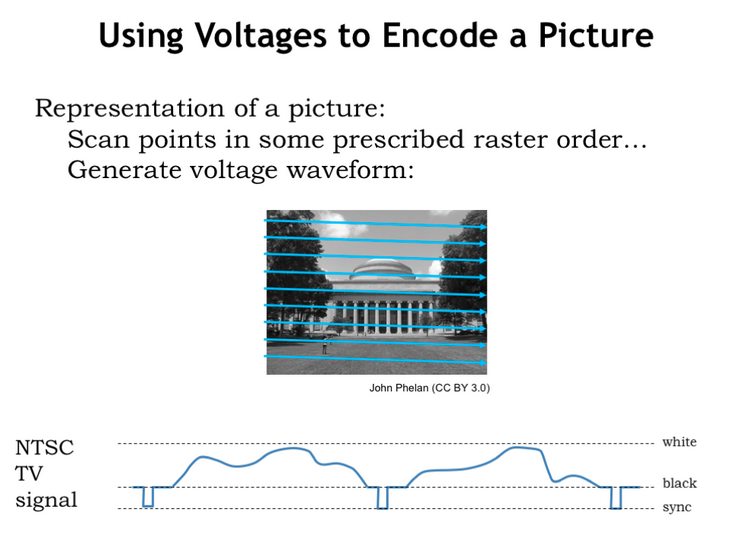
\includegraphics[scale=0.4]{assets/info_voltage1.png}
\end{center}
To complete our project of representing a complete image, we'll scan the image in some prescribed
raster order — left-to-right, top-to-bottom — converting intensities to voltages as we go.
In this way, we can convert the image into a time-varying sequence of voltages
\subsubsection{Building simple system}
Now let's see what happens when we try to build a system to process this signal. Simply reading a
picture and encoding it is static. We'll create a system using two simple processing blocks which does
things. The COPY block reproduces on its output whatever voltage appears on its input.
The output of a COPY block looks the same as the original image. The INVERTING block produces a
voltage of 1-V when the input voltage is V, i.e., white is converted to black and vice-versa.
We get the negative of the input image after passing it through an INVERTING block.
We use blocks so that we can assemble a system by connecting the blocks one to another and reason
about the behavior of the resulting system without having to understand the internal details of each block.
\begin{center}
    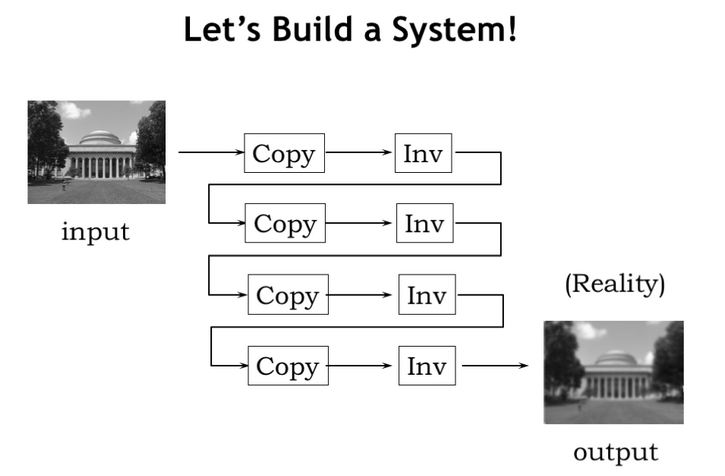
\includegraphics[scale=0.4]{assets/example_system.png}
\end{center}
So, let's build a system with our COPY and INVERTING blocks. Here's an image processing system
using a few instances each block. What do we expect the output image to look like? Well, the
COPY blocks don't change the image and there are an even number of INVERTING blocks, so, in theory,
the output image should be identical to the input image. But in reality, the output image isn't a
perfect copy of the input, it's slightly fuzzy — the intensities are slightly off and it looks like
sharp changes in intensity have been smoothed out, creating a blurry reproduction of the original.
\begin{center}
    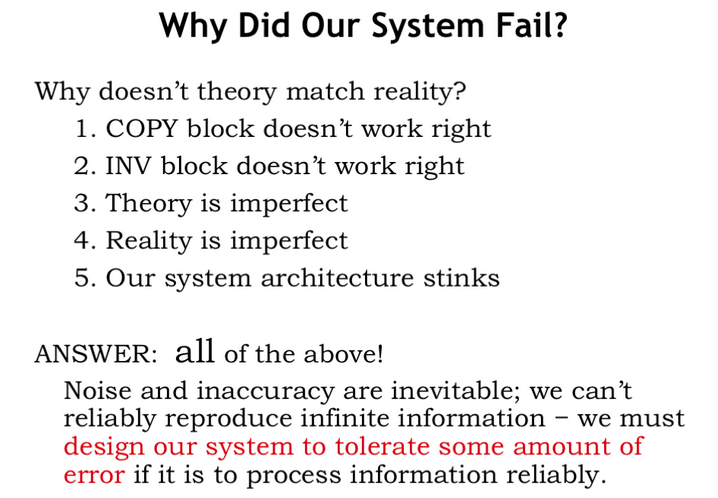
\includegraphics[scale=0.4]{assets/why_fail.png}
\end{center}
In order to mitigate this problem we shall use \textbf{digital abstraction}.

\subsubsection{Digital Abstraction}
Digital systems are designed to store, process, and communicate information in digital form.
They are found in a wide range of applications, including process control, communication systems,
digital instruments, and consumer products. The digital computer, more commonly called the computer,
is an example of a typical digital system. A computer manipulates information in digital, or more precisely,
binary form. A binary number has only two discrete values — zero or one. Each of these discrete
values is represented by the OFF and ON status of an electronic switch called a \textbf{transistor}.
\begin{center}
    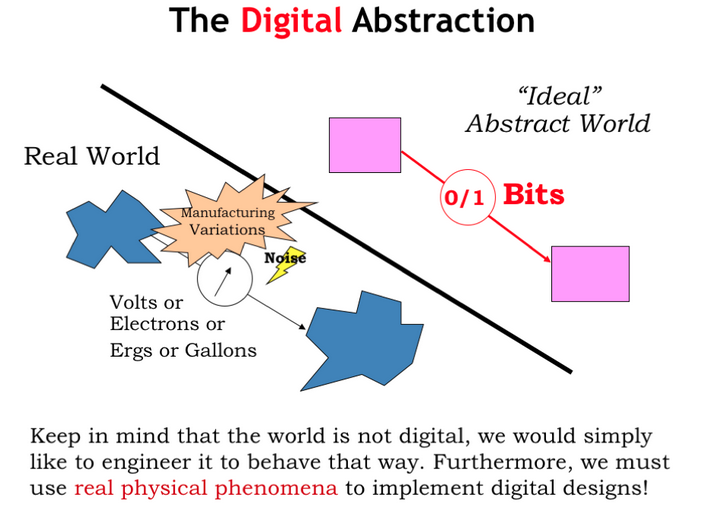
\includegraphics[scale=0.4]{assets/digital_abs.png}
\end{center}

\begin{definition}
    A signal is an electromagnetic or electrical current that is used for carrying data from one
    system or network to another. The signal is a function that conveys information about a phenomenon.
    In electronics and telecommunications, it refers to any time-varying voltage that is an
    electromagnetic wave which carries information. A signal can also be defined as an observable
    change in quality such as quantity.
\end{definition}
There are two main types of signals: Analog signal and Digital signal:
\begin{itemize}
    \item An analog signal is time-varying and generally bound to a range (e.g. +12V to -12V),
          but there is an infinite number of values within that continuous range. Analog signals are often
          calculated responses to changes in light, sound, temperature, position, pressure, or other physical
          phenomena.
    \item A digital signal is a signal that represents data as a sequence of discrete values.
          A digital signal can only take on one value from a finite set of possible values at a given time.
          Digital signals are used in all digital electronics, including computing equipment and data
          transmission    devices
\end{itemize}
To solve our engineering problem in the prevous section, we will introduce what we'll call the digital
abstraction. The key insight is to use the continuous world of voltages to represent some small,
finite set of values, in our case, the two binary values, 0 and 1. Keep in mind that the world is not
inherently digital, we would simply like to engineer it to behave that way, using continuous physical
phenomenon to implement digital designs. It'll take us three attempts to arrive at a voltage representation
 (mapped to binary bits) that solves all the problems. First two attemtps are:

\begin{center}
    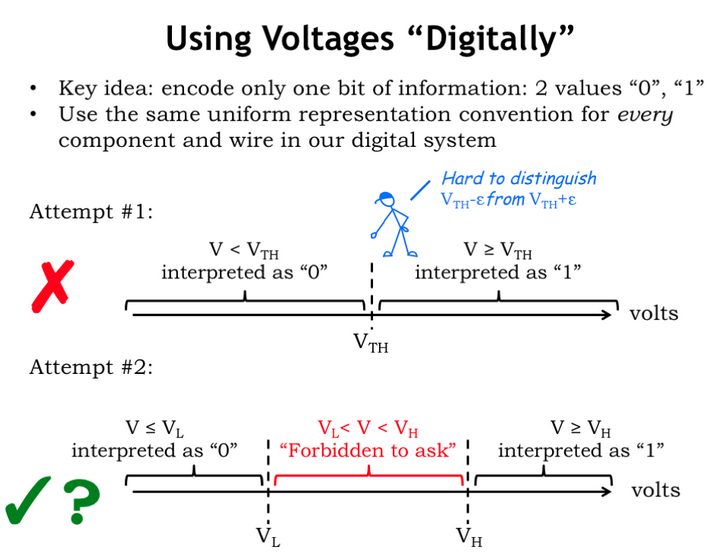
\includegraphics[scale=0.4]{assets/attemps_voltage_repr.png}
\end{center}
The second representation is pretty promising and we'll tentatively give it a green
checkmark for now. After a bit more discussion, we'll need to make one more small tweak before
we get to where we want to go.
\subsubsection{Digital Processing Elements}
We're now in a position to define our what it means to be a digital processing element.
We say a device is a \textbf{combinational device} if it meets the following four criteria:
\begin{center}
    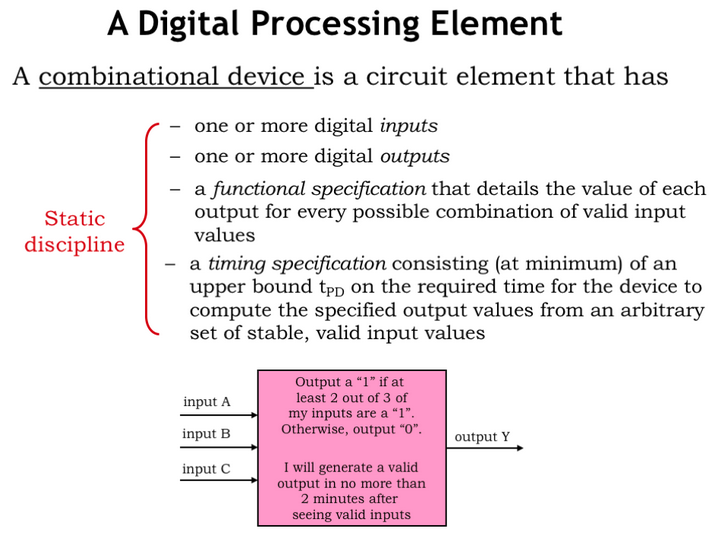
\includegraphics[scale=0.4]{assets/digital_processing_el.png}
\end{center}
\begin{definition}
    We call these four criteria \textbf{the static discipline}, which must be satisfied by all
    combinational devices.
\end{definition}
First, it should have digital inputs, by which we mean the device uses our signaling convention,
interpreting input voltages below $V_L$ (lower bound) as the digital value 0, and voltages above $V_H$
(upper bound) as the digital value 1. Second, the device's outputs should also be digital,
producing outputs of 0 by generating voltages less than or equal to and outputs of 1
by generating voltages greater than or equal to.Third, a combinational device is required to
have a functional specification that details the value of each output for every possible combination
of digital values on the inputs. Finally, a combinational device has a timing specification that tells
us how long it takes for the output of the device to reflect changes in its input values. At a minimum,
there must a specification of the propagation delay, called $t_{PD}$, that is an upper bound on the
time from when the inputs reach stable and valid digital values, to when the output is guaranteed to
have a stable and valid output value.\newline
Next we define what is a \textbf{combinational digital system}. In order to build larger combinational
systems from combinational components, we'll follow the composition rules set forth below:
\begin{itemize}
    \item each component of the system must itself be a combinational device
    \item each input of each component must be connected a system input, or to exactly one output of
          another device, or to a constant voltage representing the value 0 or the value 1
    \item the interconnected components cannot contain any directed cycles, i.e., paths through the
          system from its inputs to its outputs will only visit a particular component at most once
\end{itemize}
Our claim is that systems built using these composition rules will themselves be combinational devices.
In other words, we can build big combinational devices out of combinational components. Unlike our flaky analog system from the start of the chapter, the system can be of any size and still be expected to obey the static discipline.
\begin{proposition}
    Since the overall system does obey the static discipline and it is another combinational device.
    Thus, we can use our composition rules to build combinational devices of arbitrary complexity.
\end{proposition}
Would this digital system work?
\begin{center}
    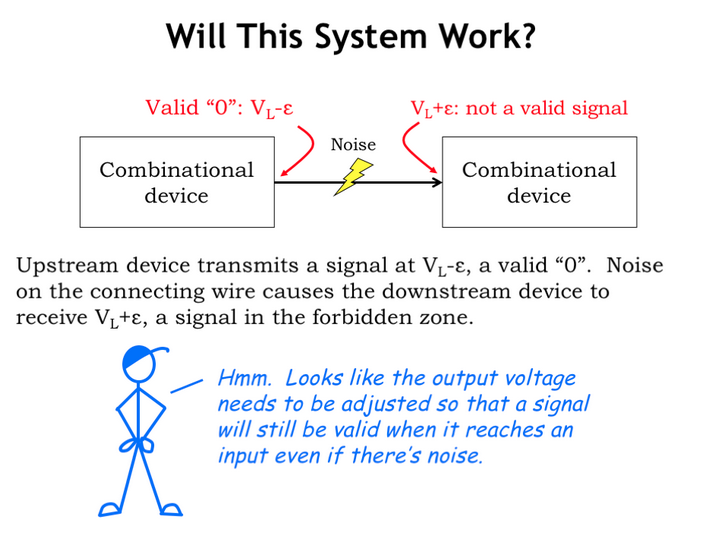
\includegraphics[scale = 0.3]{assets/will_it_work.png}
\end{center}
There's one more issue we need to deal with before finalizing our signaling specification.
Consider the following combinational system where the upstream combinational device on the left is
trying to send a digital 0 to the downstream combinational device on right. The upstream device is
generating an output voltage just slightly below $V_L$, which, according to our proposed signaling
specification, qualifies as the representation for a digital 0.
Now suppose some electrical noise slightly changes the voltage on the wire so that the voltage detected
on the input of the downstream device is slightly above $V_L$, i.e., the received signal no longer
qualifies as a valid digital input and the combinational behavior of the downstream device is no longer
guaranteed.
Oops, our system is behaving incorrectly because of some small amount of electrical noise. Just the
sort of flaky behavior we are hoping to avoid by adopting a digital systems architecture.
One way to address the problem is to adjust the signaling specification so that outputs have to obey
tighter bounds than the inputs, the idea being to ensure that valid output signals can be affected by
noise without becoming invalid input signals.

Can we avoid the problem altogether by somehow avoiding noise? A nice thought, but not a goal that we
can achieve if we're planning to use electrical components. Our proposed fix to the noise problem is to
provide separate signaling specifications for digital inputs and digital outputs:
\begin{center}
    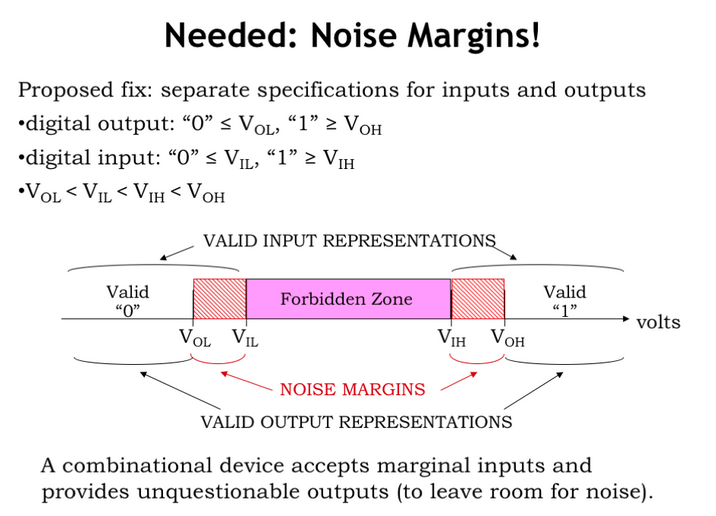
\includegraphics[scale = 0.3]{assets/noise_margins.png}
\end{center}
Combinational devices that obey this signaling specification work to remove the noise on their inputs
before it has a chance to accumulate and eventually cause signaling errors. The bottom line: digital signaling doesn't suffer from the problems we saw in our earlier analog signaling example!
\subsubsection{A Buffer example}
Let's make some measurements using one of the simplest combinational devices: a buffer. A buffer has a single
input and single output, where the output will be driven with the same digital value as the input after
some small propagation delay. This buffer obeys the static discipline — that's what it means to be
combinational — and uses our revised signaling specification that includes both low and high noise margins.
\begin{center}
    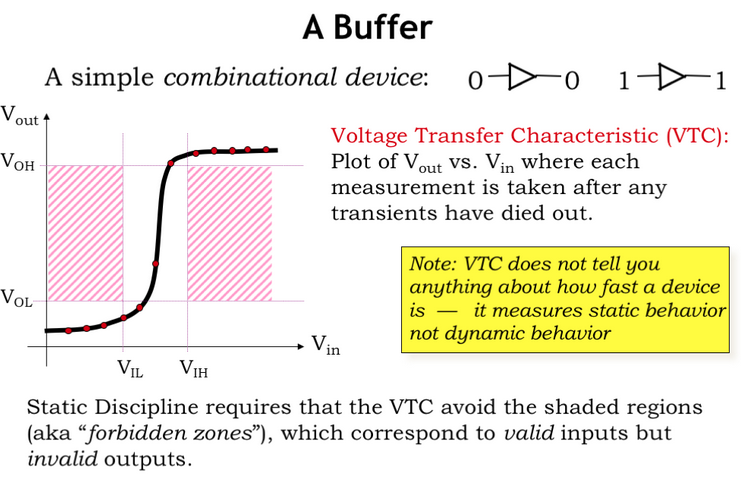
\includegraphics[scale = 0.3]{assets/buffer.png}
\end{center}
The measurements will be made by setting the input voltage to a sequence of values ranging from 0V up to
the power supply voltage. After setting the input voltage to a particular value, we'll wait for the output
voltage to become stable, i.e., we'll wait for the propagation delay of the buffer. We'll plot the result
on a graph with the input voltage on the horizontal axis and the measured output voltage on the vertical axis.
The resulting curve is called the voltage transfer characteristic of the buffer. For convenience, we've marked
our signal thresholds on the two axes.
Before we start plotting points, note that the static discipline constrains what the voltage transfer
characteristic must look like for any combinational device. If we wait for the propagation delay of the
device, the measured output voltage must be a valid digital value if the input voltage is a valid digital
value — “valid in, valid out.” We can show this graphically as shaded forbidden regions on our graph.
Points in these regions correspond to valid digital input voltages but invalid digital output voltages.
So if we're measuring a legal combinational device, none of the points in its voltage transfer characteristic
will fall within these regions.
Let's look more carefully at the white region in the center of the graph, corresponding to input voltages in
the range to $V_{IL}$ to $V_{IH}$. First note that these input voltages are in the forbidden zone of our
signaling specification and so a combinational device can produce any output voltage it likes and still
obey the static discipline, which only constrains the device's behavior for *valid* inputs.
Second, note that the center white region bounded by the four voltage thresholds is taller than it is wide.
This is true because our signaling specification has positive noise margins.
Any curve passing through this region — as the VTC must — has to have some portion where the magnitude of
the slope of the curve is greater than 1. At the point where the magnitude of the slope of the VTC is
greater than one, note that a small change in the input voltage produces a larger change in the output
voltage. That's what it means when the magnitude of the slope is greater than 1. In electrical terms,
we would say the device as a \textbf{gain greater than 1 or less than -1}, where we define gain as the
change in output voltage for a given change in input voltage.
If we're considering building larger circuits out of our combinational components, any output can
potentially be wired to some other input. This means the range on the horizontal axis ($V_{IN}$)
has to be the same as the range on the vertical axis ($V_{OUT}$), i.e., the graph of VTC must be
square and the VTC curve fits inside the square. In order to fit within the square bounds,
the VTC must change slope at some point since we know from above there must be regions where the
magnitude of the slope is greater than 1 and it can't be greater than 1 across the whole input range.
Devices that exhibit a change in gain across their operating range are called nonlinear devices.

Together these observations tell us that we cannot use only linear devices such as resistors, capacitors and inductors, to build combinational devices. We'll need nonlinear devices with gain > 1. Finding such devices is the subject of the next chapter.

\begin{center}
    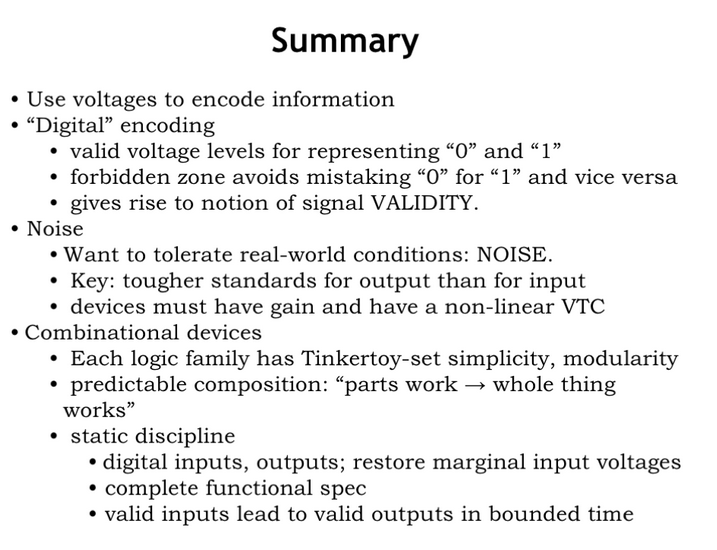
\includegraphics[scale = 0.3]{assets/summary_digital_abstraction.png}
\end{center}

Idea is that the physical representation of bits (which is just in our heads) we use voltages.
Digital abstraction for our computer is a model with discrete values.
We need to map the signal which is measured in amount of current (tok) and voltages into zeroes and ones.

We define for the input: less than  $V_{IL}$ is a zero, greater than $V_{IH}$ is a 1.
We define for output: less than $V_{OL}$ is a zero, greater than $V_{OH}$ is a 1.

For noise/error (physical machines have margin of error) we require $V_{OL} < V_{IL} < V_{IH} < V_{OH}$.
Making the output stricter (less valid values) we take care of the noise we might have in the input.

VTC Voltage Transfer Characteristic is a plot of $V_{OUT}$ vs $V_{IN}$

Gain of a combinational device is the change in output voltage for a given change in input voltage =
slope of the VTC curve.

As $V_{OH} - V_{OL} > V_{IH} - V_{IL}$ the VTC curve is very narrow within the valid input/output voltages =>
abs(gain) is greater than 1.
Overall VTC is nonlinear.
Lots of gain = big noise margins.


\subsection{Lecture 3 CMOS Technology}
Combinational device is a circuit element that has:
\begin{itemize}
    \item one or more digital inputs
    \item one or more digital outputs
    \item functional spec for the value of output for every possible combination of valid input
    \item timing spec giving upper bound on the required time for the device to compute any input
\end{itemize}

Wishlist for every combinational device:
\begin{itemize}
    \item tolerate some amount of error (noise)
    \item
\end{itemize}


\end{document}